\documentclass[12pt]{article}

\setlength{\parindent}{0pt}

% Typography
\usepackage[T1]{fontenc}
\usepackage{newtxtext,newtxmath}

% References
\usepackage[super,comma,sort&compress]{natbib}

% Mathematics
\usepackage{amsmath}
\usepackage{mathtools}
\usepackage{mathrsfs}

% Tables
\usepackage{booktabs}
\usepackage{float}
\usepackage{tabularx}

% Figures
\usepackage{graphicx}

% Layout
\usepackage[a4paper,margin=2cm]{geometry}
\usepackage{microtype}

% Section formatting
\usepackage{titlesec}

\titleformat{\section}
  {\normalfont\large\bfseries}
  {\thesection.}{0.5em}{}

\titleformat{\subsection}
  {\normalfont\normalsize\bfseries}
  {\thesubsection.}{0.5em}{}

% Code
\usepackage{xcolor}
\usepackage{listings}
\usepackage[scaled=0.92]{inconsolata}
\usepackage{tcolorbox}
\tcbuselibrary{skins,listings,xparse,breakable,hooks,theorems,fitting,raster}

\definecolor{SLcodebg}{HTML}{F7F7F7}
\definecolor{SLcodeborder}{HTML}{D9D9D9}
\definecolor{SLcodekeyword}{HTML}{2F5597}
\definecolor{SLcodestring}{HTML}{A33A3A}
\definecolor{SLcodecomment}{HTML}{5F7F5F}

\lstdefinestyle{Rstyle}{
    language=R,
    basicstyle=\ttfamily,
    keywordstyle=\color{SLcodekeyword},
    stringstyle=\color{SLcodestring},
    commentstyle=\color{SLcodecomment}\itshape,
    numbers=left,
    numberstyle=\scriptsize\color{gray},
    numbersep=6pt,
    showstringspaces=false,
    breaklines=true,
    columns=fullflexible,
    keepspaces=true,
    tabsize=2
}

\lstdefinestyle{Routput}{
    basicstyle=\ttfamily,
    numbers=none,
    showstringspaces=false,
    breaklines=true,
    columns=fullflexible,
    keepspaces=true
}

\newtcblisting[auto counter,number within=section]{rcode}[2][]{
    colback=SLcodebg,
    colframe=SLcodeborder,
    arc=1.5mm,
    boxrule=0.4pt,
    listing only,
    listing options={
        style=Rstyle,
        xleftmargin=0pt
    },
    left=5mm,
    right=2mm,
    top=2mm,
    bottom=2mm,
    enhanced,
    title={Box~\thetcbcounter.\ #2},
    fonttitle=\bfseries,
    coltitle=black,
    attach boxed title to top left={yshift=-2mm,xshift=3mm},
    boxed title style={colback=SLcodebg,colframe=SLcodeborder,boxrule=0.4pt,arc=1mm},
    #1
}

\newtcblisting{routput}{
    colback=SLcodebg,
    colframe=SLcodeborder,
    arc=1.5mm,
    boxrule=0.4pt,
    listing only,
    listing options={style=Routput},
    left=2mm,
    right=2mm,
    top=1mm,
    bottom=1mm,
    enhanced,
    title={Output~\thetcbcounter},
    fonttitle=\bfseries,
    coltitle=black,
    attach boxed title to top left={yshift=-2mm,xshift=3mm},
    boxed title style={colback=SLcodebg,colframe=SLcodeborder,boxrule=0.4pt,arc=1mm},
}

\newtcolorbox{routputbox}{
    colback=SLcodebg,
    colframe=SLcodeborder,
    arc=2mm,
    boxrule=0.4pt,
    left=3mm,
    right=3mm,
    top=2mm,
    bottom=2mm,
    enhanced,
    title={Output~\thetcbcounter},
    fonttitle=\bfseries,
    coltitle=black,
    attach boxed title to top left={yshift=-2mm,xshift=3mm},
    boxed title style={colback=SLcodebg,colframe=SLcodeborder,boxrule=0.4pt,arc=1mm},
}

% Numbered R text output
\newtcblisting[auto counter]{routputref}[1][]{
    colback=SLcodebg,
    colframe=SLcodeborder,
    arc=1.5mm,
    boxrule=0.4pt,
    listing only,
    listing options={style=Routput},
    left=2mm,
    right=2mm,
    top=1mm,
    bottom=1mm,
    enhanced,
    #1
}

% Numbered tabular R output
% Shares the same counter as routputref
\newtcolorbox[use counter from=routputref]{routputboxref}[1][]{
    colback=SLcodebg,
    colframe=SLcodeborder,
    arc=1.5mm,
    boxrule=0.4pt,
    left=3mm,
    right=3mm,
    top=2mm,
    bottom=2mm,
    enhanced,
    #1
}

% Caption below the output
\newcommand{\routputcaption}[2]{%
    \par\smallskip
    \begin{center}
        Box~\ref{#1}: #2
    \end{center}
}

% Links
\usepackage[hidelinks]{hyperref}

\title{\textbf{Super Learner: A Practical Tutorial}}
\author{}
\date{}

\title{\textbf{Super Learner: A Practical Tutorial}}
\author{}
\date{}

\begin{document}

\maketitle

\begin{abstract}
The selection of an optimal predictive model is a pervasive challenge in biostatistics and epidemiology. Relying on a single \textit{a priori} algorithm risks overfitting and reduced generalizability when applied to new settings. Super Learner is a flexible ensemble machine-learning method that mitigates these risks by combining multiple candidate algorithms into a single prediction model. Using cross-validation, it defines a weighted combination of learners that minimizes a specified loss function, ensuring performance asymptotically equal to or better than the best candidate algorithm. This tutorial provides a comprehensive, practical guide to implementing Super Learner in R for applied researchers. Using a simulated epidemiological dataset with a binary outcome, we demonstrate the step-by-step construction of the ensemble. We cover the foundational statistical concepts, basic implementation, evaluation through cross-validation, hyperparameter tuning, feature screening, and performance optimization for metrics such as the Area Under the ROC Curve (AUC). Additionally, we detail advanced usage, including computational parallelization and the integration of custom algorithms and screening procedures. This guide equips epidemiologists and clinical researchers with the tools necessary to confidently incorporate robust machine-learning techniques into their predictive modeling workflows.
\end{abstract}

\noindent\textbf{Keywords:} Super Learner; ensemble learning; cross-validation; statistical learning.

\section{Introduction}

A common challenge in the use of predictive models is that their performance may deteriorate when they are applied outside the conditions, populations, or settings in which they were developed and evaluated \cite{Collinse074819}. This behavior may arise from multiple factors, including shifts in the data distribution or population characteristics that were not adequately represented during model training \cite{Zhang2022Shifting}. In addition, the relative performance of learning methods may vary according to the characteristics and structure of the data; therefore, an algorithm that performs well under certain conditions may not necessarily retain that advantage in other settings \cite{ALI2006119,Uddin2024}. This dependence makes the \textit{a priori} selection of a single method difficult and may lead to increasingly complex model specifications in an attempt to adapt the model to the available data, thereby increasing the risk of overfitting and capturing sample-specific variation rather than generalizable patterns \cite{Pavlou2016}. \\
In clinical settings, the appropriate selection and evaluation of predictive models is particularly important because their predictions may contribute to clinical decision-making. An overfitted model may exhibit apparently strong performance in the data used for its development but show reduced predictive ability when applied to new individuals, resulting in overly optimistic estimates of its performance \cite{Riley2020,Collins2024}. \\
Super Learner (SL) is an ensemble learning algorithm that combines predictions from multiple candidate algorithms with the aim of improving predictive performance. Using a library of models with different structures and degrees of flexibility, SL relies on cross-validation to evaluate their performance and estimate a weighted combination that minimizes a specified loss function. This procedure allows the predictive strengths of different algorithms to be leveraged without relying on the \textit{a priori} selection of a single model \cite{vanDerLaan2007}. \\
This tutorial provides a practical guide to the implementation and use of Super Learner for epidemiologists, biostatisticians, and clinical researchers interested in incorporating machine-learning methods into their analyses. Through a progressive presentation of its foundations, implementation, and interpretation, the tutorial aims to provide the elements required to construct and evaluate models using Super Learner and to identify the main methodological decisions involved in its application.

\section{Super Learner Fundamentals}
Super Learner is an ensemble machine-learning method that uses $V$-fold cross-validation to estimate the performance of a set of candidate algorithms. Based on these estimates, it determines a weighted combination of their predictions by optimizing a loss function, to obtain a predictor whose performance is asymptotically at least as good as that of the best candidate algorithm in the library \cite{vanDerLaan2007}.

\subsection{Statistical Foundations}
In a clinical study, a vector of covariates ($W_i$) and an outcome ($Y_i$) are observed for each individual $i$. The observed data for each individual can be represented as

\begin{equation}
    O_i = (W_i, Y_i), \qquad i = 1, \ldots, n.
\end{equation}

The observations are assumed to arise from the same data-generating process, represented by an unknown probability distribution $P_0$, such that

\begin{equation}
    O_1,\ldots,O_n \overset{\mathrm{i.i.d.}}{\sim} P_0.
\end{equation}

The prediction problem consists of estimating a function $\psi$ that maps covariate values to a prediction of the outcome:

\begin{equation}
    \psi: \mathcal{W} \rightarrow \mathbb{R}.
\end{equation}

Here, $\psi(w)$ denotes the prediction corresponding to the covariate values $W=w$.
Prediction rules are compared using a loss function $L$. The risk of a prediction rule is defined as its expected loss:

\begin{equation}
    R(\psi) = E_{P_0}\left[L\left(Y,\psi(W)\right)\right].
\end{equation}

The expectation is taken with respect to the true data-generating distribution $P_0$.
The optimal prediction rule, with respect to the specified loss function, is defined as the rule that minimizes the expected risk:

\begin{equation}
    \psi_0 = \arg\min_{\psi} R(\psi).
\end{equation}

\subsection{Estimation Procedure}
Super Learner starts from a collection of candidate learning algorithms. Let $\mathcal{A}_k$, for $k=1,\ldots,K$, denote a learning algorithm that, when trained on a data set, produces a fitted prediction rule $\widehat{\psi}_k$. The collection of candidate algorithms defines the library

\begin{equation}
    \mathcal{L} = \left\{\mathcal{A}_1,\ldots,\mathcal{A}_K\right\}.
\end{equation}

Because the true distribution $P_0$ is unknown, the population risk $R(\psi)$ cannot be evaluated directly. Super Learner therefore uses cross-validation to estimate the predictive performance of the candidate algorithms and determine their combination within the ensemble.
To implement $V$-fold cross-validation, the $n$ observations are divided into $V$ subsets. For each iteration $v=1,\ldots,V$, let $V(v)$ denote the validation set and $T(v)$ its complementary training set. Each candidate algorithm $\mathcal{A}_k$ is fitted using $T(v)$ and generates predictions for the observations contained in $V(v)$. Because these predictions are obtained from models that were not fitted using the corresponding validation observations, they constitute cross-validated, or \textit{out-of-fold}, predictions.
The predictions obtained from the $K$ candidate algorithms are collected in an $n \times K$ matrix $Z$,

\begin{equation}
    Z = (Z_1,\ldots,Z_K),
\end{equation}

where $Z_k$ contains the cross-validated predictions obtained from algorithm $\mathcal{A}_k$.
Given the matrix $Z$, Super Learner combines the predictions of the candidate algorithms using a set of weights. Let $\alpha=(\alpha_1,\ldots,\alpha_K)$ denote the vector of weights assigned to the $K$ candidate algorithms. These weights are estimated through a meta-learning procedure, referred to as the \textit{meta-learner}, which seeks the combination that minimizes the cross-validated risk:

\begin{equation}
    \widehat{\alpha}
    =
    \arg\min_{\alpha} R_{CV}(\alpha).
\end{equation}

Here, $R_{CV}(\alpha)$ denotes the risk associated with the weighted combination defined by $\alpha$.
The specific form of this criterion depends on the meta-learning procedure used to estimate the ensemble weights. For the standard convex combination, the weights satisfy

\begin{equation}
    \alpha_k \geq 0,
    \qquad
    \sum_{k=1}^{K} \alpha_k = 1.
\end{equation}

Once the weights have been estimated, each candidate algorithm is refitted using the full sample. For a new set of covariate values $w$, the final Super Learner prediction is defined as

\begin{equation}
    \widehat{\psi}_{SL}(w)
    =
    \sum_{k=1}^{K}
    \widehat{\alpha}_k
    \widehat{\psi}_k(w).
\end{equation}

\section{Super Learner in Epidemiology and Biostatistics}
The following table summarizes several practical motivations for using Super Learner in biostatistical and epidemiological applications.

\begin{table}[H]
\centering
\caption{Practical applications of Super Learner in epidemiology and biostatistics.}
\label{tab:sl_applications}
\begin{tabularx}{\textwidth}{p{0.42\textwidth} X}
\toprule
\textbf{Challenge} & \textbf{Contribution of Super Learner} \\
\midrule
Uncertainty about the best model & Weighted ensemble of multiple candidate algorithms. \\
Risk of overfitting with complex models & Cross-validated risk estimation. \\
High-dimensional covariates & Variable selection through incorporated \textit{screeners}. \\
Binary, continuous, and survival outcomes & Flexible specification according to the type of outcome. \\
Reproducibility & Seed-controlled procedures and reproducible data partitions. \\
From prediction to causal inference & Application in the estimation of components required by TMLE and AIPW. \\
\bottomrule
\end{tabularx}
\end{table}

\section{Practical Implementation of Super Learner}
In R, Super Learner is available through the \texttt{SuperLearner} package \cite{vanDerLaan2007}. 
To reproduce the examples presented throughout this tutorial, additional packages 
are required alongside the core package. These packages provide some of the 
candidate algorithms, tools for performance evaluation, and auxiliary functions 
used throughout the analysis.\\
Packages in R can be installed using the \texttt{install.packages()} function. 
This operation downloads the packages from CRAN and adds them to the local R 
installation, so it generally needs to be performed only once for each working 
environment.

\begin{rcode}[label={code:install}]{Installing required packages}
# Core package
install.packages("SuperLearner")

# Packages used throughout this tutorial
install.packages(c(
  "glmnet", "randomForest", "ranger", "xgboost", "earth", "gam",
  "gbm", "rpart", "nnet", "e1071", "ipred", "ada",
  "ggplot2", "ROCR", "pROC", "caret", "data.table", "mlbench",
  "RhpcBLASctl", "rmutil", "vcd", "nnls", "Matrix"
))
\end{rcode}

The first command (Box~\ref{code:install}) installs the core \texttt{SuperLearner} package, whereas the second installs additional packages \cite{Friedman2010, Liaw2002, Wright2017, Chen2016, Hastie1990, Hastie2017, Ridgeway1999, Therneau1997, Ripley1996} that will later be used to incorporate 
different candidate algorithms, perform variable screening and transformation, 
evaluate predictive performance, and implement some of the extensions presented 
in the tutorial. The specific role of each package will be introduced as it is 
used. \\
Once installed, the \texttt{SuperLearner} package must be loaded into the current 
R session using (Box~\ref{code:load-sl}):

\begin{rcode}[label={code:load-sl}]{Loading the SuperLearner package}
library(SuperLearner)
\end{rcode}

\subsection{Simulated Epidemiological Data}
This tutorial is developed using a simulated data set. The data represent an 
epidemiological setting with a binary outcome, such as the presence or absence 
of disease, and a set of covariates related to the outcome through linear effects, 
interactions, and nonlinear relationships. Because the data-generating mechanism 
is known, the behavior of Super Learner can be evaluated under a controlled and 
predefined structure. \\
A total of $n=500$ observations and five covariates $(W_1,\ldots,W_5)$ are 
generated. The first four covariates are drawn from uniform distributions and 
illustratively represent standardized characteristics such as age, body mass 
index, blood pressure, and a biomarker. The fifth covariate, $W_5$, represents a 
binary comorbidity indicator whose probability depends on $W_2$ and $W_3$.

\begin{rcode}[label={code:sim-covariates}]{Generating simulated covariates}
set.seed(2743)
n <- 500

# Covariates (standardised to unit scale)
W1 <- runif(n, 0.5, 1)
W2 <- runif(n, 0, 1)
W3 <- runif(n, 0.25, 0.75)
W4 <- runif(n, 0, 1)

# A derived comorbidity indicator
W5 <- rbinom(n, 1, 1 / (1 + exp(1.5 * W2 - W3)))
\end{rcode}

The binary outcome $Y$ is generated using a logistic model that includes main 
effects, an interaction between $W_5$ and $W_1$, and a nonlinear term involving 
$W_4$. Consequently, the data-generating mechanism represents a structure that 
is more complex than a purely linear relationship between the covariates and 
the outcome.

\begin{rcode}[label={code:sim-outcome}]{Generating the binary outcome}
# True data-generating mechanism: interactions + non-linearity
logit_p <- -0.2 * W5 - 2 * W1 + 4 * W5 * W1 - 1.5 * W2 + sin(W4 * pi)
Y <- rbinom(n, 1, 1 / (1 + exp(-logit_p)))

dat <- data.frame(W1, W2, W3, W4, W5, Y)
\end{rcode}

Once the data have been generated, the resulting distribution of the simulated 
sample can be examined. Because the outcome $Y$ is binary, its mean corresponds 
to the proportion of observations for which $Y=1$, and therefore provides the 
prevalence of the simulated outcome. In addition, \texttt{summary()} provides 
an initial descriptive summary of the generated variables.

\begin{rcode}[label={code:descriptive}]{Descriptive summary of the simulated data}
cat("Prevalence of the outcome:", round(mean(Y), 3), "\n")
summary(dat)
\end{rcode}

\begin{routputboxref}[label={box:summary}]
	\centering
	\ttfamily
	
	\begin{tabular}{lrrrrrr}
		& W1     & W2      & W3     & W4      & W5    & Y    \\
		Min.      & 0.500  & 0.00056 & 0.252  & 0.00388 & 0.000 & 0.00 \\
		1st Qu.   & 0.615  & 0.24025 & 0.372  & 0.24555 & 0.000 & 0.00 \\
		Median    & 0.728  & 0.47032 & 0.502  & 0.49973 & 0.000 & 0.00 \\
		Mean      & 0.740  & 0.47600 & 0.495  & 0.50607 & 0.436 & 0.44 \\
		3rd Qu.   & 0.864  & 0.72776 & 0.618  & 0.76426 & 1.000 & 1.00 \\
		Max.      & 0.999  & 0.99765 & 0.750  & 0.99940 & 1.000 & 1.00 \\
	\end{tabular}
	
\end{routputboxref}

To further examine the distribution of the simulated binary outcome, a bar plot can be used as an additional descriptive tool:

\begin{figure}[H]
    \centering
    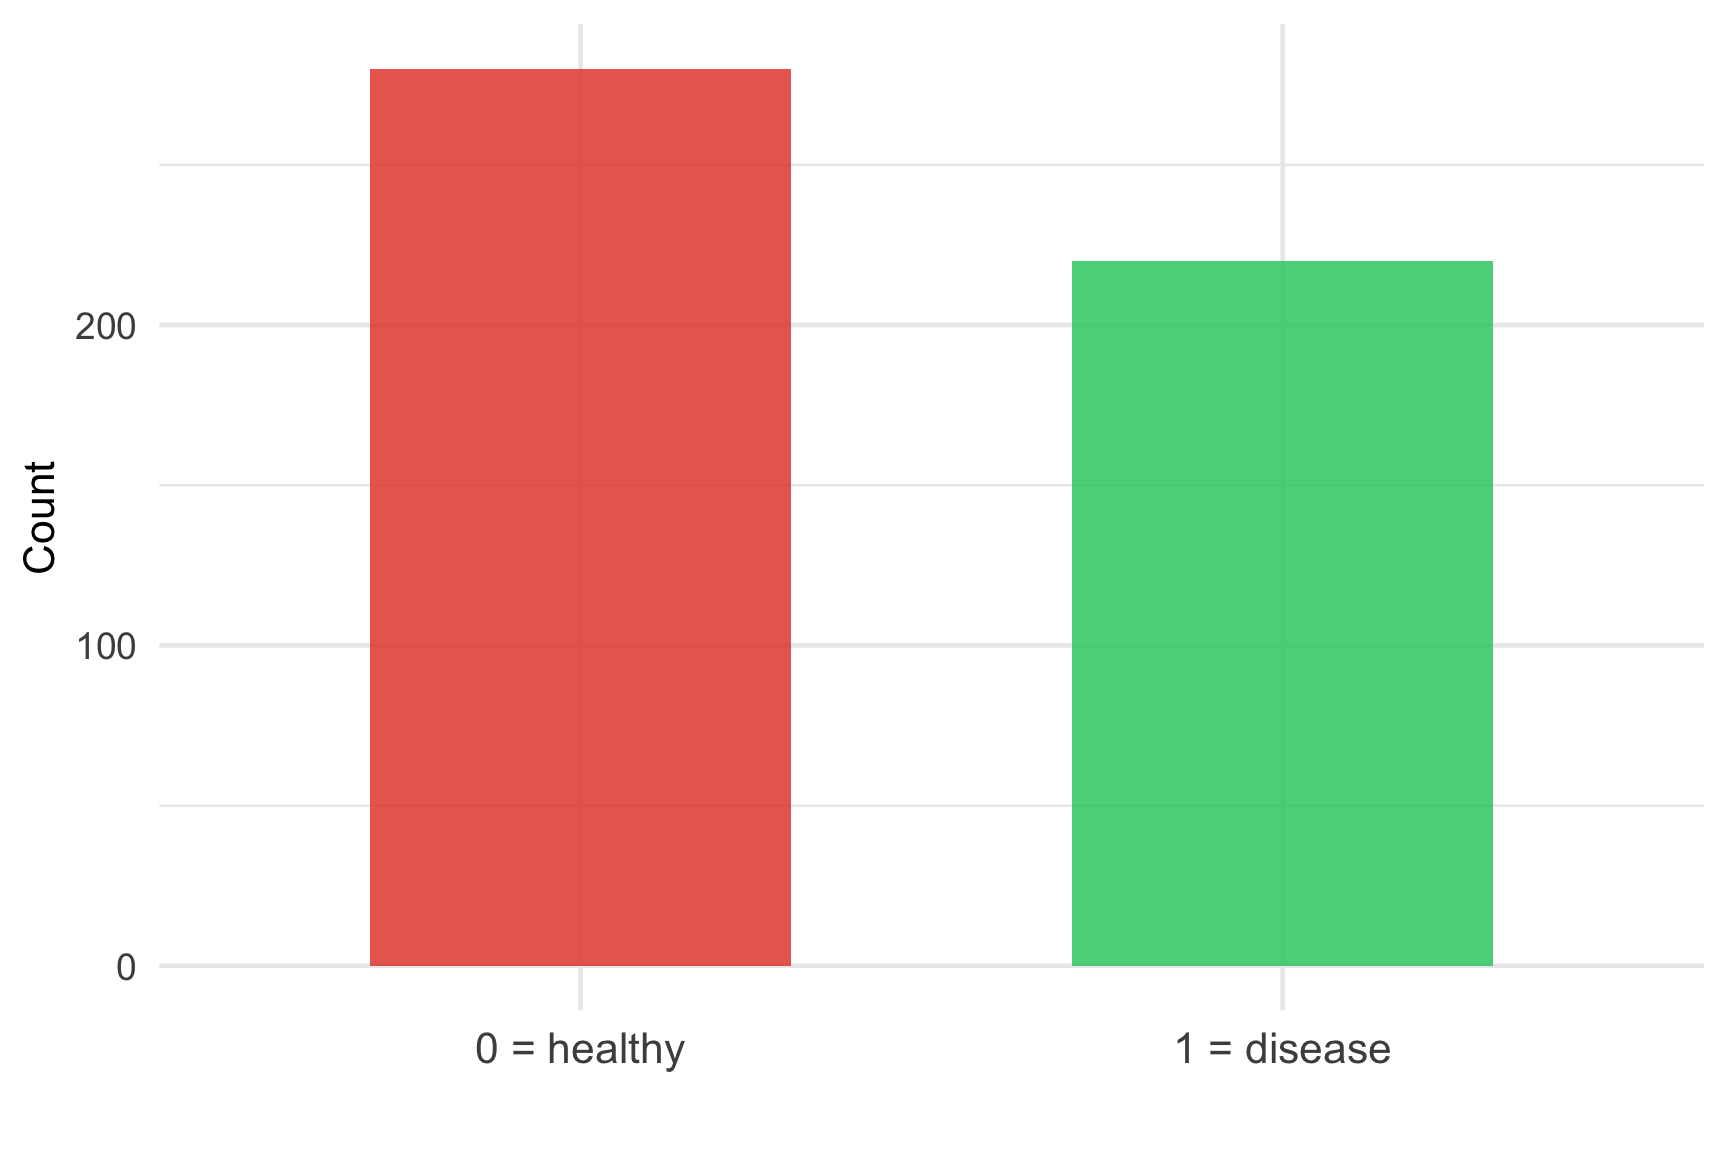
\includegraphics[width=0.5\linewidth]{OUT_1.png}
    \caption{Distribution of the simulated binary outcome.}
    \label{fig:outcome_distribution}
\end{figure}

A total of 44\% of the simulated observations have the outcome of interest, 
corresponding to the presence of disease ($Y=1$), while the covariates remain 
within the ranges specified during data generation. These data will subsequently 
be used to progressively evaluate the performance of different candidate 
algorithms and their combination through Super Learner.

\section{Basic Super Learner}

The first practical approach to Super Learner begins with a single candidate algorithm, 
with the aim of familiarizing the reader with the \texttt{SuperLearner()} function 
and the main elements of its output. Additional algorithms are subsequently incorporated 
into the library to examine how Super Learner assigns weights among the candidates 
according to their cross-validated performance.

\subsection{A Single Algorithm}

The first fit uses penalized logistic regression through LASSO/elastic net, implemented 
in Super Learner using \texttt{SL.glmnet}. The simulated data are divided into two sets: 
80\% of the observations are used for training and the remaining 20\% are reserved for 
testing. To preserve the same partition in subsequent analyses, the random seed is fixed 
using \texttt{set.seed(123)} (Box~\ref{code:sl-single}).

\begin{rcode}[label={code:sl-single}]{Fitting Super Learner with a single algorithm}
set.seed(123)

# Train / test split (80 % / 20 %)
train_idx <- sample(1:n, 400)
X_train   <- dat[train_idx, 1:5]
Y_train   <- dat[train_idx, 6]
X_test    <- dat[-train_idx, 1:5]
Y_test    <- dat[-train_idx, 6]

sl_lasso <- SuperLearner(
  Y = Y_train, X = X_train,
  family = binomial(),
  SL.library = "SL.glmnet"
)
sl_lasso
\end{rcode}

The output of \texttt{sl\_lasso} reports two main elements: the risk estimated through 
cross-validation (\texttt{Risk}) and the weight assigned to the algorithm (\texttt{Coef}). 
In this first fit, the weight is equal to 1 because the library contains only 
\texttt{SL.glmnet}, and therefore there are no other algorithms among which the weight 
can be distributed. Although these results are presented together in the general output, 
they can also be accessed separately using \texttt{sl\_lasso\$cvRisk} and 
\texttt{sl\_lasso\$coef}.

\begin{routputboxref}[label={box:sl-single}]
	\ttfamily
	\raggedright
	
	Call:
	
	SuperLearner(
	Y = Y\_train,
	X = X\_train,
	family = binomial(),
	SL.library = "SL.glmnet"
	)
	
	\medskip
	
	\centering
	\begin{tabular}{lrr}
		& Risk & Coef \\
		SL.glmnet\_All & 0.1612 & 1 \\
	\end{tabular}
\end{routputboxref}

\routputcaption{box:sl-single}
{Super Learner fit with a single candidate algorithm.}

To examine the model fitted by \texttt{SL.glmnet}, the coefficients corresponding to 
each covariate can be extracted at the penalty value selected by cross-validation 
(\texttt{lambda.min}) using Box~\ref{code:lasso-coef}:

\begin{rcode}[label={code:lasso-coef}]{Extracting LASSO coefficients}
round(as.matrix(coef(fit_lasso, s = "lambda.min")), 3)
\end{rcode}

The resulting output is:

\begin{routputboxref}[label={box:lasso-coefficients}]
	\ttfamily
	\centering
	\begin{tabular}{lr}
		& lambda.min \\
		(Intercept) & -1.478 \\
		W1          &  0.183 \\
		W2          & -0.778 \\
		W3          &  0.004 \\
		W4          &  0.652 \\
		W5          &  2.545 \\
	\end{tabular}
\end{routputboxref}

\routputcaption{box:lasso-coefficients}
{Coefficients estimated by \texttt{SL.glmnet} at \texttt{lambda.min}.}

The result of this first approach will serve as a reference for comparing the changes 
observed as additional algorithms are incorporated into the library.

\subsection{Two Algorithms}
For the second fit (Box~\ref{code:sl-two}), \texttt{SL.randomForest} is added to the library while retaining the algorithm used in the previous case (\texttt{SL.glmnet}). Super Learner therefore estimates a combination of both candidates and assigns a weight to each according to its performance within the cross-validation procedure.

\begin{rcode}[label={code:sl-two}]{Fitting Super Learner with two algorithms}
set.seed(123)

sl_two <- SuperLearner(
  Y = Y_train, X = X_train,
  family = binomial(),
  SL.library = c("SL.glmnet", "SL.randomForest")
)
sl_two
\end{rcode}

\begin{routputboxref}[label={box:sl-two}]
	\ttfamily
	\raggedright
	
	Call:
	
	SuperLearner(
	Y = Y\_train, X = X\_train, family = binomial(),
	SL.library = c("SL.glmnet", "SL.randomForest")
	)
	
	\medskip
	
	\centering
	\begin{tabular}{lrr}
		& Risk & Coef \\
		SL.glmnet\_All       & 0.1593 & 0.7003 \\
		SL.randomForest\_All & 0.1661 & 0.2997 \\
	\end{tabular}
\end{routputboxref}

\routputcaption{box:sl-two}
{Super Learner fit with two candidate algorithms.}

After incorporating a second algorithm, the weight is no longer concentrated on a single candidate and is instead distributed between the two models. In the previous fit, \texttt{SL.glmnet} received a weight of 1; in this case, its weight decreases to $0.7003$, while \texttt{SL.randomForest} receives the remaining weight. This output shows that both algorithms contribute to the ensemble, although with different weights.

\subsection{A Full Ensemble with a Reference Model}
A reference model is a simple model used as a point of comparison to assess whether 
more complex models provide an improvement in predictive performance. In this case, 
\texttt{SL.mean} is added to the library. This learner predicts the sample mean of the 
outcome. Because the outcome is binary, this prediction corresponds to the observed 
prevalence and is the same for all individuals. Owing to its simplicity and low 
computational cost, it provides a useful reference for assessing the contribution of 
the other algorithms in the library.

\begin{rcode}[label={code:sl-reference}]{Including a reference model in the ensemble}
set.seed(123)
sl <- SuperLearner(
  Y = Y_train, X = X_train,
  family = binomial(),
  SL.library = c("SL.mean", "SL.glmnet", "SL.randomForest")
)
sl
\end{rcode}

\begin{routputboxref}[label={box:sl-reference}]
	\ttfamily
	\raggedright
	
	Call:
	
	SuperLearner(
	Y = Y\_train, X = X\_train, family = binomial(),
	SL.library = c("SL.mean", "SL.glmnet", "SL.randomForest")
	)
	
	\medskip
	
	\centering
	\begin{tabular}{lrr}
		& Risk & Coef \\
		SL.mean\_All         & 0.2478 & 0.0000 \\
		SL.glmnet\_All       & 0.1593 & 0.7003 \\
		SL.randomForest\_All & 0.1661 & 0.2997 \\
	\end{tabular}
\end{routputboxref}

\routputcaption{box:sl-reference}
{Super Learner fit including the reference model.}

The output shows that \texttt{SL.mean} receives a weight of $0$ and therefore does 
not contribute to the ensemble prediction. The weights assigned to 
\texttt{SL.glmnet} and \texttt{SL.randomForest} remain nearly identical to those 
obtained in the previous two-algorithm fit, indicating that both algorithms continue 
to make a relevant contribution to the ensemble. \\
As additional information, the computational time required for model fitting can be 
examined using \texttt{sl\$times\$everything}. This quantity provides a simple way to 
monitor computational cost as the number of algorithms included in the library 
increases.

\begin{rcode}[label={code:sl-time}]{Checking computational time}
# Time it took to fit
sl$times$everything
\end{rcode}

\begin{routputref}[label={box:sl-time}]
	user  system elapsed 
	4.993   0.184   5.219 
\end{routputref}

\routputcaption{box:sl-time}
{Computational time required to fit the Super Learner ensemble.}

\section{Predictions and Performance}

Once the ensemble has been fitted and the weights of its component algorithms have 
been estimated, the 20\% of the data previously reserved as a test set is used to 
generate predictions and evaluate predictive performance.

\subsection{Generating Predictions}

The \texttt{predict()} function uses the fitted ensemble to generate predictions for 
new data. In this case, both the final Super Learner prediction and the individual 
predictions generated by each algorithm in the library are retained. To obtain both 
types of predictions, the argument \texttt{onlySL = FALSE} is specified.

\begin{rcode}[label={code:predict}]{Generating predictions on the test set}
# Keep ensemble and individual learner predictions
pred <- predict(sl, newdata = X_test, onlySL = FALSE)
str(pred)
\end{rcode}

\begin{routputref}[label={box:prediction-structure}]
	List of 2
	$ pred           : num [1:100, 1] 0.205 0.146 0.174 0.707 0.258 ...
	$ library.predict: num [1:100, 1:3] 0.44 0.44 0.44 0.44 0.44 0.44 0.44 0.44 0.44 0.44 ...
	..- attr(*, "dimnames")=List of 2
	.. ..$ : NULL
	.. ..$ : chr [1:3] "SL.mean_All" "SL.glmnet_All" "SL.randomForest_All"
\end{routputref}

\routputcaption{box:prediction-structure}{Structure of the prediction object returned by \texttt{predict()}.}

The resulting object contains two components. \texttt{pred\$pred} stores the final 
ensemble predictions, whereas \texttt{pred\$library.predict} contains the predictions 
generated by each candidate algorithm. In this case, 100 predictions are generated, 
corresponding to the observations included in the test set.

The first ensemble predictions can be examined using (Box~\ref{code:head-pred}):

\begin{rcode}[label={code:head-pred}]{Examining ensemble predictions}
# Ensemble predictions (probability of disease)
head(pred$pred)
\end{rcode}

\begin{routputboxref}[label={box:ensemble-predictions}]
	\ttfamily
	\centering
	\begin{tabular}{lr}
		& {[,1]} \\
		{[1,]} & 0.2050 \\
		{[2,]} & 0.1459 \\
		{[3,]} & 0.1736 \\
		{[4,]} & 0.7068 \\
		{[5,]} & 0.2584 \\
		{[6,]} & 0.1671 \\
	\end{tabular}
\end{routputboxref}

\routputcaption{box:ensemble-predictions}
{First predicted probabilities generated by the Super Learner ensemble.}

Each value corresponds to the predicted probability of the outcome for an observation 
in the test set. For example, for the first observation, the ensemble estimates a 
probability of approximately $0.205$.

The predictions generated individually by the algorithms in the library can be 
examined in the same way (Box~\ref{code:head-library}):

\begin{rcode}[label={code:head-library}]{Examining individual learner predictions}
# Predictions from each individual learner
head(pred$library.predict)
\end{rcode}

\begin{routputboxref}[label={box:individual-predictions}]
	\ttfamily
	\centering
	\begin{tabular}{lrrr}
		& SL.mean\_All & SL.glmnet\_All & SL.randomForest\_All \\
		{[1,]} & 0.44 & 0.2636 & 0.068 \\
		{[2,]} & 0.44 & 0.1493 & 0.138 \\
		{[3,]} & 0.44 & 0.1785 & 0.162 \\
		{[4,]} & 0.44 & 0.7653 & 0.570 \\
		{[5,]} & 0.44 & 0.2111 & 0.369 \\
		{[6,]} & 0.44 & 0.2173 & 0.050 \\
	\end{tabular}
\end{routputboxref}

\routputcaption{box:individual-predictions}
{First predicted probabilities generated by the individual candidate algorithms.}

To examine the distribution of the probabilities predicted by the ensemble, these 
can be displayed according to the observed outcome in the test set. 
Figure~\ref{fig:predicted_probabilities} shows the distribution of the estimated 
probabilities for individuals without and with disease.

\begin{figure}[H]
    \centering
    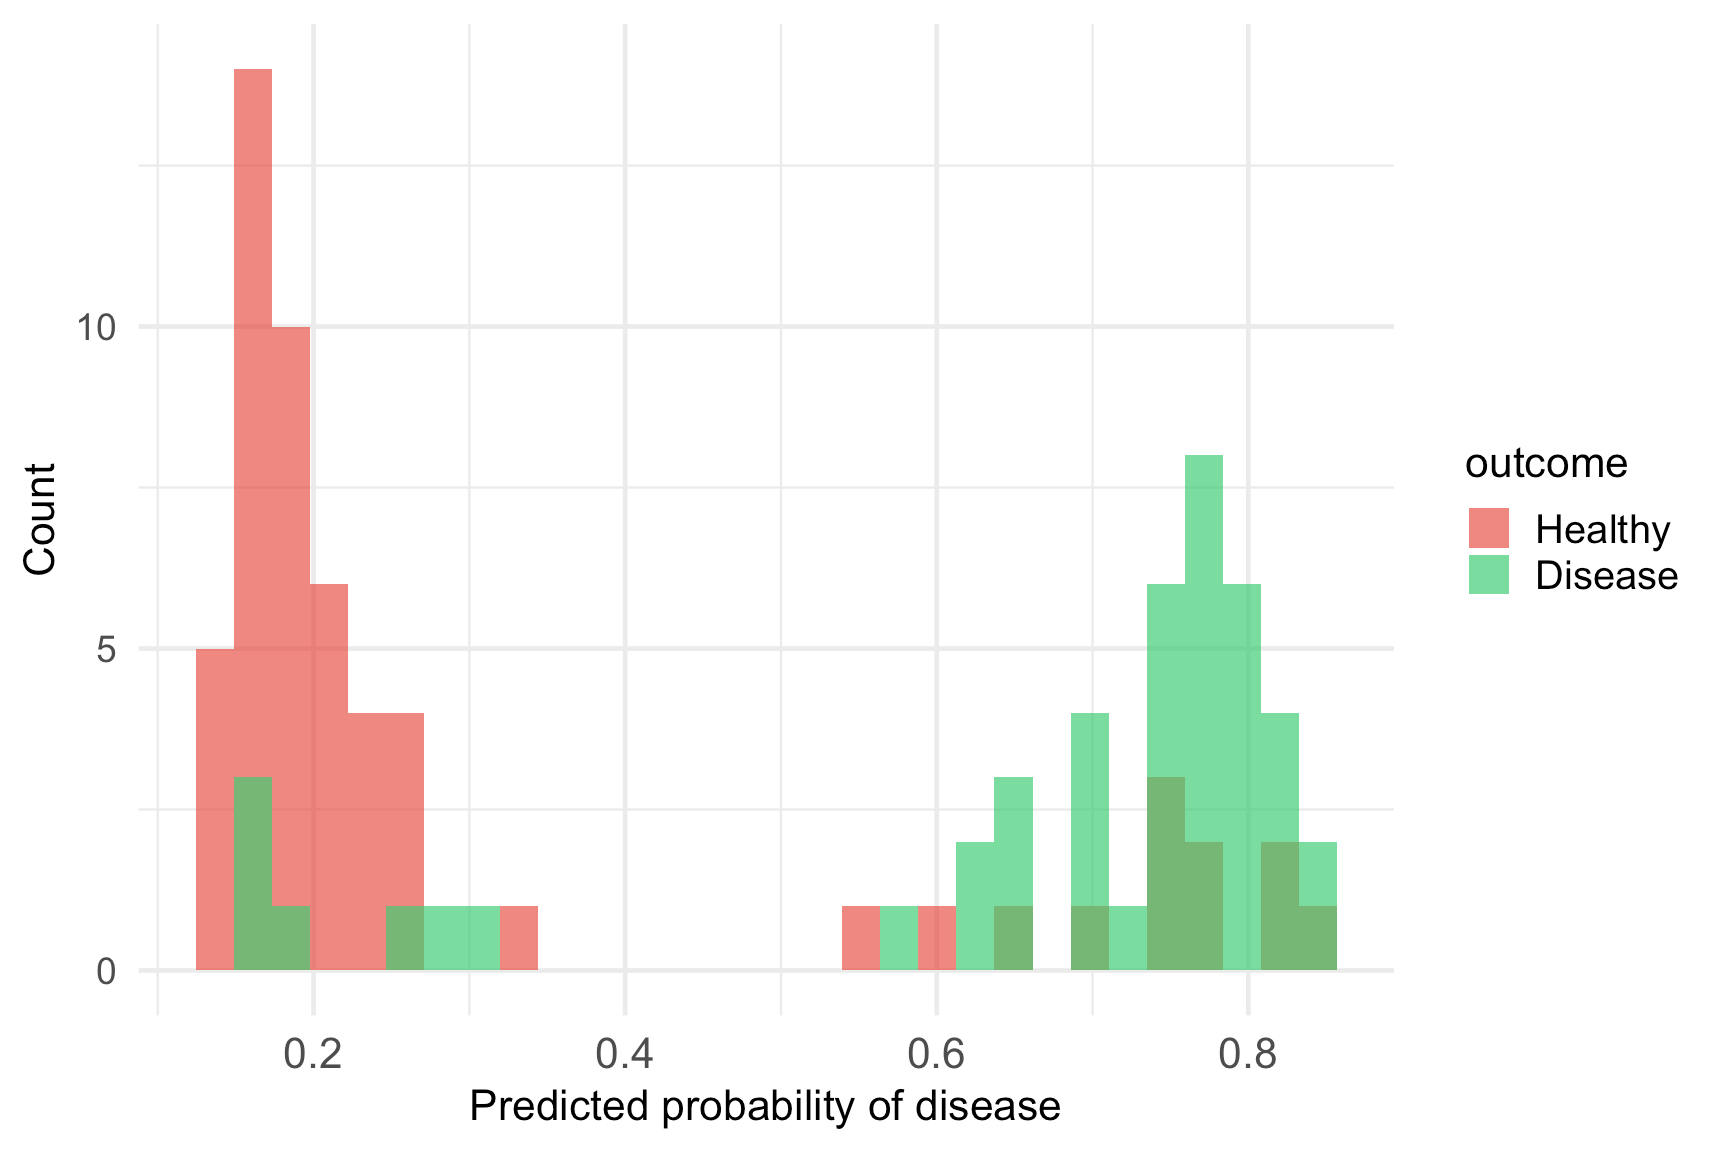
\includegraphics[width=0.85\linewidth]{pred_1.png}
    \caption{Predicted probabilities by true outcome.}
    \label{fig:predicted_probabilities}
\end{figure}

The predicted probabilities for individuals without disease are concentrated mainly 
at lower values, whereas those for individuals with disease are concentrated at 
higher values. Although some overlap is present between the two distributions, a 
degree of separation between the groups can be observed, suggesting that the ensemble 
has discriminatory ability between individuals with and without the outcome.

\subsection{Area Under the ROC Curve}

The discriminatory ability of Super Learner can be summarized using the area under the ROC curve (AUC). This measure evaluates the ability of the model to assign higher predicted probabilities to individuals with the outcome than to those without the outcome. Values close to $0.5$ indicate limited discrimination, whereas values approaching $1$ reflect greater discriminatory ability.

In this case, the AUC is calculated using the predictions obtained on the test set (Box~\ref{code:auc}):

\begin{rcode}[label={code:auc}]{Computing the AUC on the test set}
pred_rocr <- ROCR::prediction(pred$pred, Y_test)

auc_sl <- ROCR::performance(
  pred_rocr,
  measure = "auc",
  x.measure = "cutoff"
)@y.values[[1]]

cat("Test AUC:", round(auc_sl, 4), "\n")
\end{rcode}

\begin{routputref}[label={box:test-auc}]
	Test AUC: 0.8417
\end{routputref}

\routputcaption{box:test-auc}
{Area under the ROC curve for the Super Learner ensemble on the test set.}

Super Learner achieves an AUC of $0.8417$ on the test set, indicating an ability to discriminate between individuals with and without the outcome.

To compare the ensemble with the individual algorithms, the AUC and ROC curve are also calculated for each candidate in the library (Box~\ref{code:roc-curves}). This allows the performance of \texttt{SL.mean}, \texttt{SL.glmnet}, \texttt{SL.randomForest}, and Super Learner to be examined jointly.

\begin{rcode}[label={code:roc-curves}]{ROC curves for the ensemble and individual algorithms}
# Column order of library.predict matches SL.library:
#  1 = SL.mean, 2 = SL.glmnet, 3 = SL.randomForest
auc_mean   <- pROC::auc(Y_test, pred$library.predict[, 1])
auc_glmnet <- pROC::auc(Y_test, pred$library.predict[, 2])
auc_rf     <- pROC::auc(Y_test, pred$library.predict[, 3])

roc_mean   <- pROC::roc(Y_test, pred$library.predict[, 1], quiet = TRUE)
roc_glmnet <- pROC::roc(Y_test, pred$library.predict[, 2], quiet = TRUE)
roc_rf     <- pROC::roc(Y_test, pred$library.predict[, 3], quiet = TRUE)
roc_sl     <- pROC::roc(Y_test, pred$pred, quiet = TRUE)

roc_df <- data.frame(
  FPR   = c(1 - roc_mean$specificities, 1 - roc_glmnet$specificities,
            1 - roc_rf$specificities, 1 - roc_sl$specificities),
  TPR   = c(roc_mean$sensitivities, roc_glmnet$sensitivities,
            roc_rf$sensitivities, roc_sl$sensitivities),
  Model = rep(c(
    paste0("Mean (AUC = ", round(auc_mean, 3), ")"),
    paste0("LASSO (AUC = ", round(auc_glmnet, 3), ")"),
    paste0("Random Forest (AUC = ", round(auc_rf, 3), ")"),
    paste0("SuperLearner (AUC = ", round(auc_sl, 3), ")")
  ), times = sapply(list(roc_mean, roc_glmnet, roc_rf, roc_sl),
                    function(x) length(x$sensitivities)))
)

ggplot(roc_df, aes(x = FPR, y = TPR, color = Model)) +
  geom_line(size = 1.1) +
  geom_abline(intercept = 0, slope = 1, linetype = "dashed",
              color = "gray50") +
  scale_color_manual(values = c("#3498DB", "#E74C3C", "#9B59B6", "#2ECC71")) +
  labs(x = "1 - Specificity", y = "Sensitivity") +
  xlim(0, 1) + ylim(0, 1) +
  theme_minimal(base_size = 14) +
  theme(legend.position = c(0.65, 0.25))
\end{rcode}

\begin{figure}[H]
    \centering
    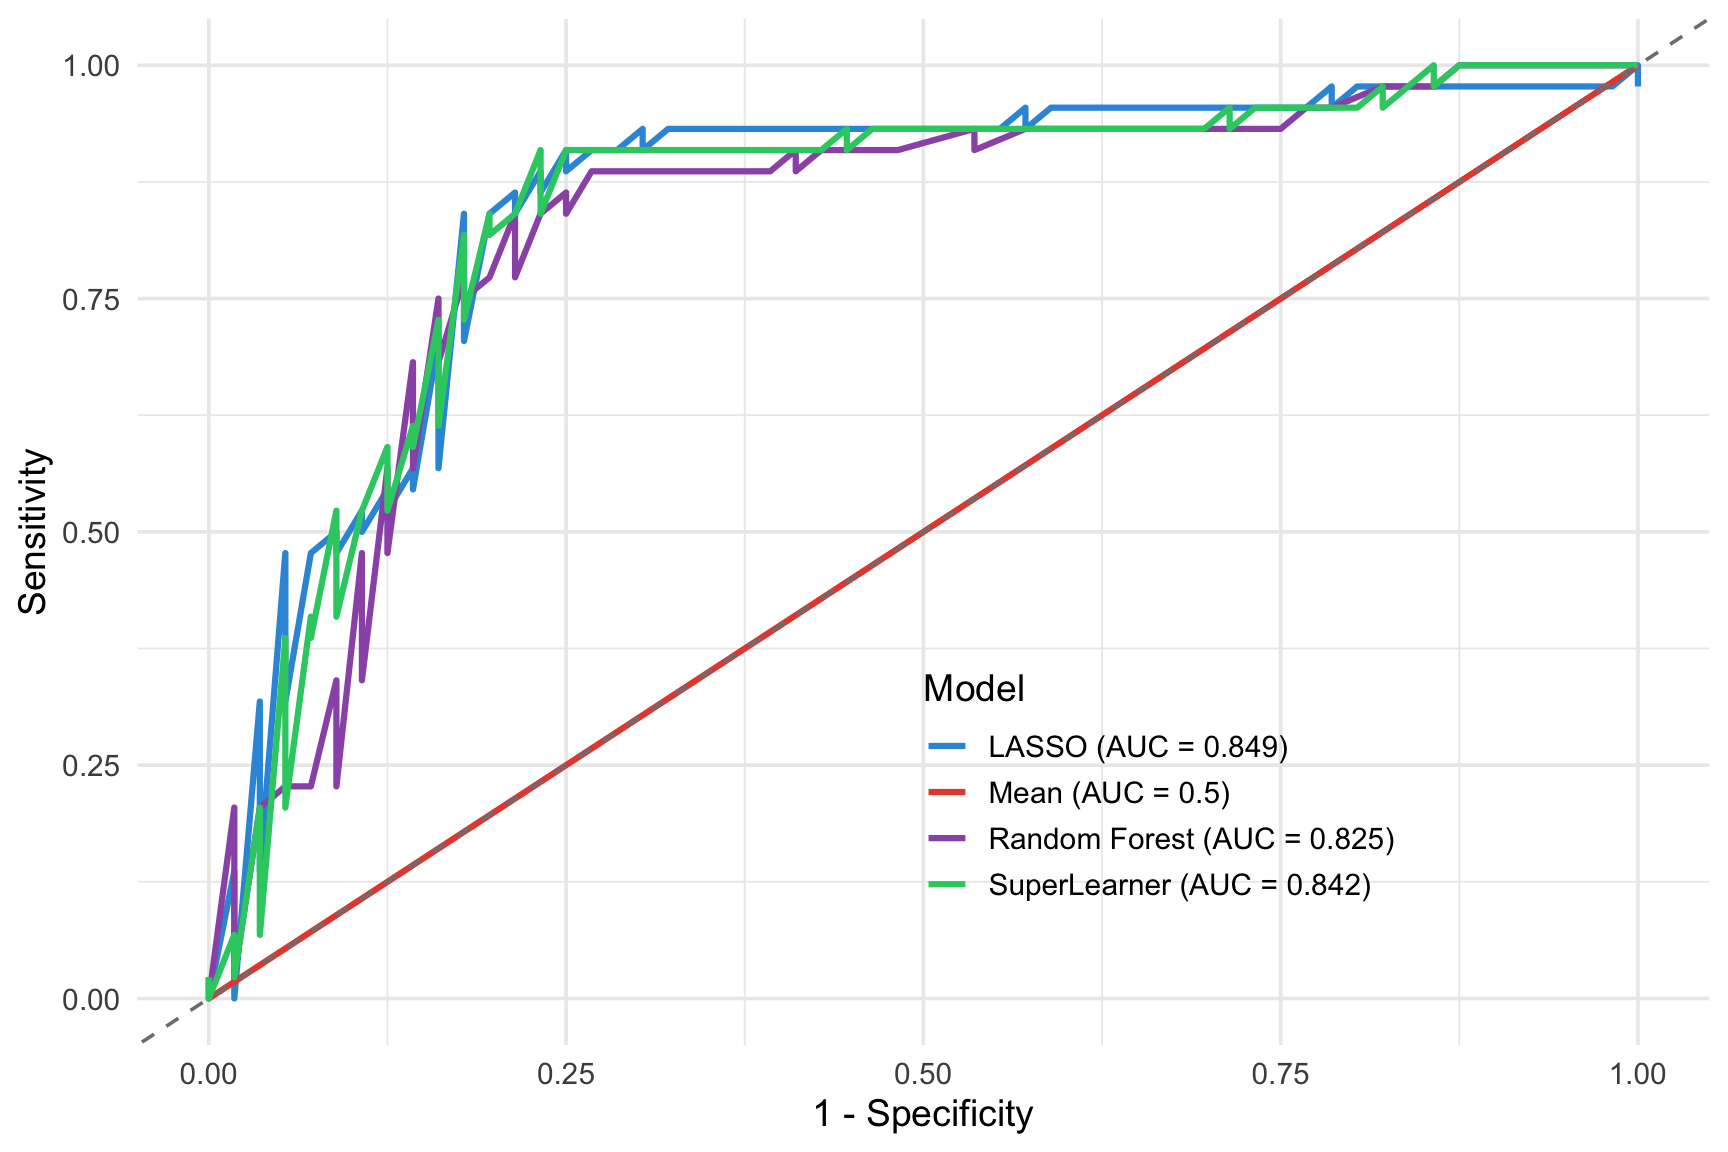
\includegraphics[width=0.85\linewidth]{multi_roc.png}
    \caption{ROC curves for Super Learner and the individual candidate algorithms.}
    \label{fig:pla_mul}
\end{figure}

Figure~\ref{fig:pla_mul} shows the differences in discriminatory performance among the evaluated models. Because \texttt{SL.mean} generates a constant prediction for all observations, it lies on the reference line. In contrast, \texttt{SL.glmnet}, \texttt{SL.randomForest}, and Super Learner show greater ability to distinguish between individuals with and without the outcome.

Super Learner achieves an AUC of $0.842$, comparable to that observed for the individual algorithms with the highest discriminatory performance in this test set.


\section{Cross-Validated Super Learner}
Up to this point, the performance of Super Learner has been evaluated using a single training-test split. Although this strategy allows the model to be assessed on observations that were not used during fitting, the resulting estimates correspond to one specific partition of the data. Cross-validation complements this analysis by evaluating the procedure across different partitions and summarizing both its average performance and its variability. \\
In this context, a distinction should be made between the internal cross-validation used to estimate the risk of the candidate algorithms and determine the ensemble weights, and the external cross-validation implemented through \texttt{CV.SuperLearner()}, which is used to evaluate the complete procedure. In each external partition, Super Learner is refitted using the corresponding training data and evaluated on observations that were not used in that fit.

\subsection{Fitting \texttt{CV.SuperLearner}} 
In this example, the 400 observations in the training set are divided into five partitions of 80 observations each. At each iteration, 320 observations are used to refit Super Learner, including its internal cross-validation procedure, while the remaining 80 observations are used to evaluate its risk. The process is repeated until each partition has served once as the external evaluation set.

\begin{rcode}[label={code:cvsl}]{Fitting CV.SuperLearner}
set.seed(123)

system.time({
  cv_sl <- CV.SuperLearner(
    Y = Y_train, X = X_train,
    family = binomial(),
    V = 5,
    SL.library = c("SL.mean", "SL.glmnet", "SL.randomForest")
  )
})
\end{rcode}

\begin{routputref}[label={box:cvsl-time}]
	user  system elapsed 
	18.365   1.016  19.751 
\end{routputref}

\routputcaption{box:cvsl-time}
{Computational time required to fit \texttt{CV.SuperLearner()}.}

The summary of the \texttt{cv\_sl} object allows the risk obtained across the five external partitions to be examined for both Super Learner and the individual algorithms in the library:

\begin{rcode}[label={code:cvsl-summary}]{Summarizing CV.SuperLearner results}
summary(cv_sl)
\end{rcode}

\begin{routputboxref}[label={box:cvsl-summary}]
	\ttfamily
	Call:\par
	CV.SuperLearner(Y = Y\_train, X = X\_train, V = 5, family = binomial(),
	SL.library = c("SL.mean", "SL.glmnet", "SL.randomForest"))\par
	
	\medskip
	Risk is based on: Mean Squared Error\par
	
	\medskip
	All risk estimates are based on V = 5\par
	
	\medskip
	\centering
	\begin{tabular}{lrrrr}
		Algorithm & Ave & se & Min & Max \\
		Super Learner        & 0.16 & 0.0115 & 0.13 & 0.21 \\
		Discrete SL          & 0.16 & 0.0116 & 0.13 & 0.22 \\
		SL.mean\_All         & 0.25 & 0.0031 & 0.24 & 0.27 \\
		SL.glmnet\_All       & 0.16 & 0.0116 & 0.13 & 0.22 \\
		SL.randomForest\_All & 0.17 & 0.0119 & 0.15 & 0.22 \\
	\end{tabular}
\end{routputboxref}

\routputcaption{box:cvsl-summary}
{Cross-validated risk summary for Super Learner and the candidate algorithms.}

In this case, risk is expressed using the mean squared error. The \texttt{Ave} column corresponds to the average risk obtained across the five external partitions, \texttt{se} to its standard error, and \texttt{Min} and \texttt{Max} to the observed range across partitions. The \textit{Super Learner} row summarizes the performance of the full ensemble, whereas \textit{Discrete SL} corresponds to the best individual candidate algorithm; this comparison makes it possible to assess whether the weighted combination provides an improvement over selecting a single candidate. \\
Super Learner achieves an average risk of $0.16$, which is nearly identical to that observed for \texttt{SL.glmnet} and Discrete SL. \texttt{SL.randomForest} shows a slightly higher risk, whereas \texttt{SL.mean} has the highest value. Figure~\ref{fig:cv_risk} displays these estimates together with their 95\% confidence intervals.

\begin{figure}[H]
    \centering
    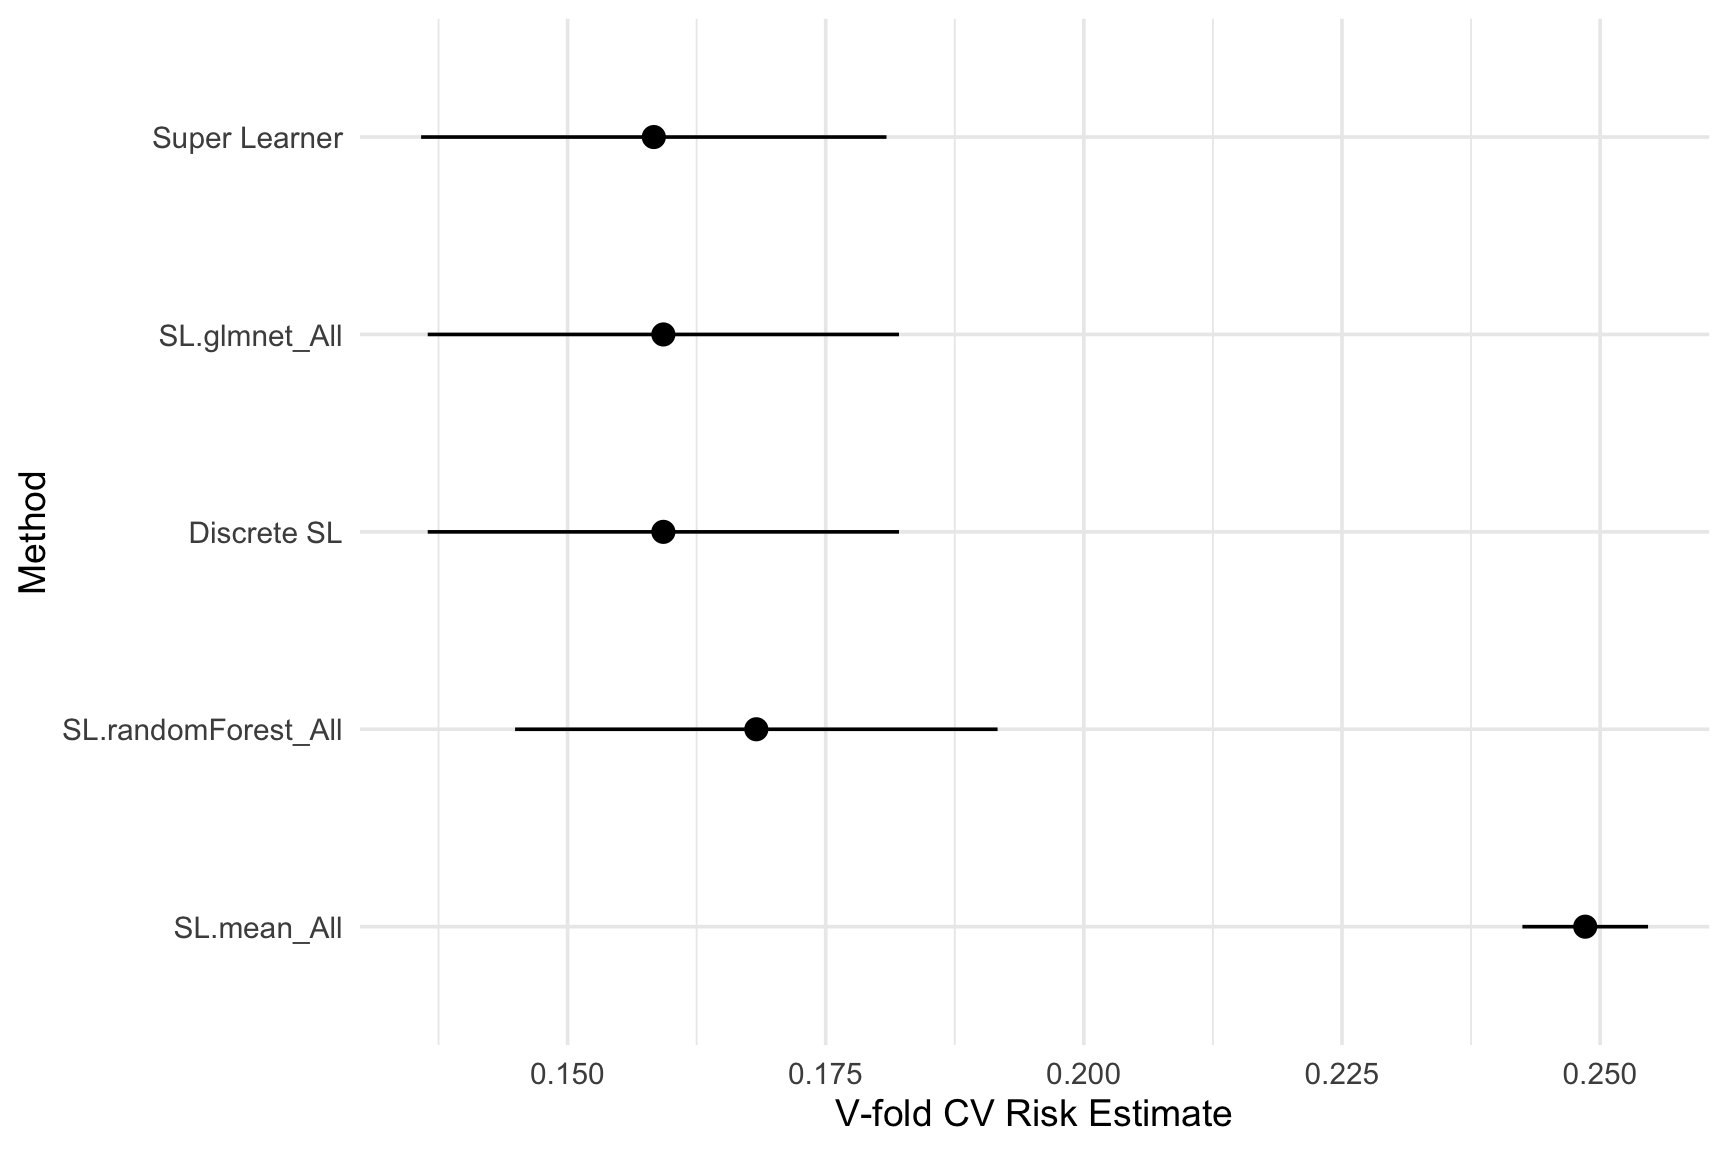
\includegraphics[width=0.85\linewidth]{plot_cv_SL.png}
    \caption{Cross-validated risk (mean squared error) with 95\% confidence intervals.}
    \label{fig:cv_risk}
\end{figure}

Figure~\ref{fig:cv_risk} shows that the risk estimates for Super Learner, Discrete SL, and \texttt{SL.glmnet} are concentrated at very similar values, whereas \texttt{SL.mean} is clearly shifted toward higher risk. The intervals for the methods with lower risk show substantial overlap, although this pattern should not by itself be interpreted as formal evidence of equivalent performance. \\
Para identificar qué algoritmo candidato corresponde al \textit{Discrete SL} en cada partición externa, puede examinarse el objeto \texttt{cv\_sl\$whichDiscreteSL} (Box~\ref{code:discrete-sl}):

\begin{rcode}[label={code:discrete-sl}]{Identifying the Discrete Super Learner}
table(simplify2array(cv_sl$whichDiscreteSL))
\end{rcode}

\begin{routputref}[label={box:discrete-sl-selection}]
	SL.glmnet_All 
	5 
\end{routputref}

\routputcaption{box:discrete-sl-selection}
{Best individual candidate selected across the external cross-validation folds.}

En las cinco particiones externas, \texttt{SL.glmnet} fue el algoritmo candidato con menor riesgo. Esto explica que el riesgo del \textit{Discrete SL} sea prácticamente idéntico al observado para \texttt{SL.glmnet} en el resumen anterior. Aunque este algoritmo fue seleccionado como el mejor candidato individual en todas las particiones, el Super Learner mantiene una combinación ponderada de los candidatos, aspecto que puede examinarse mediante la distribución de los pesos entre particiones.

\subsection{Distribution of Ensemble Weights}
In addition to identifying the best individual candidate, it is useful to examine how the ensemble weights vary across the external cross-validation folds. This makes it possible to assess whether the weighting pattern observed in a single fit remains similar when the composition of the training data changes.

\begin{rcode}[label={code:review-weights}]{Distribution of ensemble weights across folds}
	review_weights <- function(cv_sl) {
		meta_weights <- coef(cv_sl)              # matrix: folds x learners
		means <- colMeans(meta_weights)
		sds   <- apply(meta_weights, 2, sd)
		mins  <- apply(meta_weights, 2, min)
		maxs  <- apply(meta_weights, 2, max)
		stats <- cbind("mean(weight)" = means, sd = sds, min = mins, max = maxs)
		stats[order(stats[, 1], decreasing = TRUE), ]
	}
	
	print(review_weights(cv_sl), digits = 3)
\end{rcode}

\begin{routputboxref}[label={box:weight-distribution}]
	\ttfamily
	\centering
	\begin{tabular}{lrrrr}
		Algorithm & mean(weight) & sd & min & max \\
		SL.glmnet\_All       & 0.768 & 0.0499 & 0.694 & 0.819 \\
		SL.randomForest\_All & 0.232 & 0.0499 & 0.181 & 0.306 \\
		SL.mean\_All         & 0.000 & 0.0000 & 0.000 & 0.000 \\
	\end{tabular}
\end{routputboxref}

\routputcaption{box:weight-distribution}
{Distribution of ensemble weights across the external cross-validation folds.}

As shown in Box~\ref{box:weight-distribution}, \texttt{SL.glmnet} receives the largest average weight ($0.768$), followed by \texttt{SL.randomForest} ($0.232$), whereas \texttt{SL.mean} receives a weight of $0$ in all folds. This pattern is consistent with the previous results, in which \texttt{SL.glmnet} showed the best performance among the individual candidate algorithms. \\
The variation in the weights across folds is relatively small. For \texttt{SL.glmnet}, the weights range from $0.694$ to $0.819$, whereas for \texttt{SL.randomForest} they range from $0.181$ to $0.306$. In this example, the distribution of the weights remains broadly similar across the five external cross-validation folds.

\section{Hyperparameter Tuning}

Up to this point, each algorithm has been incorporated into the library using a single configuration. However, many algorithms depend on hyperparameters that can modify their predictive behavior. In Super Learner, different configurations of the same algorithm can be incorporated as distinct candidates and evaluated using the same cross-validation procedure introduced previously.

\subsection{Algorithm Variants}

Random Forest provides a useful example of this possibility. One of its hyperparameters is \texttt{ntree}, which determines the number of trees used. Until now, \texttt{SL.randomForest} has been used with its default configuration. To evaluate an alternative with 3000 trees, a \textit{wrapper} can be defined (Box~\ref{code:rf-wrapper}):

\begin{rcode}[label={code:rf-wrapper}]{Random Forest variant with custom wrapper}
	SL.rf.better <- function(...) {
		SL.randomForest(..., ntree = 3000)
	}
	
	set.seed(123)
	
	cv_sl_rf <- CV.SuperLearner(
	Y = Y_train, X = X_train,
	family = binomial(),
	V = 5,
	SL.library = c(
	"SL.mean",
	"SL.glmnet",
	"SL.rf.better",
	"SL.randomForest"
	)
	)
	
	summary(cv_sl_rf)
\end{rcode}

\begin{routputboxref}[label={box:rf-trees}]
	\ttfamily
	\centering
	\begin{tabular}{lrrrr}
		Algorithm & Ave & se & Min & Max \\
		Super Learner & 0.16 & 0.0115 & 0.13 & 0.21 \\
		Discrete SL & 0.16 & 0.0117 & 0.13 & 0.22 \\
		SL.mean\_All & 0.25 & 0.0031 & 0.24 & 0.27 \\
		SL.glmnet\_All & 0.16 & 0.0117 & 0.13 & 0.22 \\
		SL.rf.better\_All & 0.17 & 0.0119 & 0.15 & 0.22 \\
		SL.randomForest\_All & 0.17 & 0.0120 & 0.15 & 0.22 \\
	\end{tabular}
\end{routputboxref}

\routputcaption{box:rf-trees}
{Cross-validated risk after including two Random Forest configurations.}

The variant with 3000 trees has a risk that is nearly identical to that of the \texttt{SL.randomForest} configuration used previously. In this example, increasing the number of trees does not produce an appreciable improvement in predictive performance.

When only a single configuration needs to be modified, a \textit{wrapper} is sufficient. To generate variants automatically, \texttt{create.Learner()} can be used (Box~\ref{code:create-learner}):

\begin{rcode}[label={code:create-learner}]{Generating a variant with create.Learner}
	learners <- create.Learner(
	"SL.randomForest",
	params = list(ntree = 3000)
	)
	
	learners$names
\end{rcode}

\begin{routputref}[label={box:create-learner-name}]
	[1] "SL.randomForest_1"
\end{routputref}

\routputcaption{box:create-learner-name}
{Random Forest variant generated by \texttt{create.Learner()}.}

The function generates a new candidate that retains \texttt{SL.randomForest} while modifying the specified value of \texttt{ntree}. This approach is particularly useful when several configurations need to be evaluated.

\subsection{Hyperparameter Grids}

The evaluation can be extended to several values of a hyperparameter. In Random Forest, \texttt{mtry} determines the number of variables considered as candidates at each split. With the five covariates used in this example, the reference value is (Box~\ref{code:mtry-default}):

\begin{rcode}[label={code:mtry-default}]{Reference value of mtry}
	floor(sqrt(ncol(X_train)))
\end{rcode}

\begin{routputref}[label={box:mtry-default}]
	[1] 2
\end{routputref}

\routputcaption{box:mtry-default}
{Reference value of \texttt{mtry} for the simulated data.}

Based on this value, three \texttt{mtry} configurations are generated (Box~\ref{code:mtry-grid}):

\begin{rcode}[label={code:mtry-grid}]{Generating mtry configurations}
	mtry_seq <- floor(
	sqrt(ncol(X_train)) * c(0.5, 1, 2)
	)
	
	learners_mtry <- create.Learner(
	"SL.randomForest",
	tune = list(mtry = mtry_seq)
	)
	
	learners_mtry$names
\end{rcode}

\begin{routputref}[label={box:mtry-learners}]
	[1] "SL.randomForest_1" "SL.randomForest_2" "SL.randomForest_3"
\end{routputref}

\routputcaption{box:mtry-learners}
{Random Forest candidates generated for different values of \texttt{mtry}.}

These variants can be incorporated directly into the library (Box~\ref{code:cvsl-mtry}):

\begin{rcode}[label={code:cvsl-mtry}]{Evaluating mtry configurations with CV.SuperLearner}
	set.seed(123)
	
	cv_sl_mtry <- CV.SuperLearner(
	Y = Y_train, X = X_train,
	family = binomial(),
	V = 5,
	SL.library = c(
	"SL.mean",
	"SL.glmnet",
	learners_mtry$names,
	"SL.randomForest"
	)
	)
	
	summary(cv_sl_mtry)
\end{rcode}

\begin{routputboxref}[label={box:mtry-summary}]
	\ttfamily
	\centering
	\begin{tabular}{lrrrr}
		Algorithm & Ave & se & Min & Max \\
		Super Learner & 0.16 & 0.0118 & 0.13 & 0.21 \\
		Discrete SL & 0.16 & 0.0120 & 0.13 & 0.22 \\
		SL.mean\_All & 0.25 & 0.0031 & 0.24 & 0.27 \\
		SL.glmnet\_All & 0.16 & 0.0116 & 0.13 & 0.22 \\
		SL.randomForest\_1\_All & 0.16 & 0.0126 & 0.13 & 0.21 \\
		SL.randomForest\_2\_All & 0.17 & 0.0120 & 0.15 & 0.22 \\
		SL.randomForest\_3\_All & 0.17 & 0.0129 & 0.15 & 0.23 \\
		SL.randomForest\_All & 0.17 & 0.0119 & 0.15 & 0.22 \\
	\end{tabular}
\end{routputboxref}

\routputcaption{box:mtry-summary}
{Cross-validated risk for the Random Forest hyperparameter configurations.}

The Random Forest configurations show similar risk values, although \texttt{SL.randomForest\_1} achieves an average risk of $0.16$, compared with approximately $0.17$ for the configuration used previously. This result illustrates that different configurations of the same algorithm can exhibit different predictive performance and can therefore be included as candidates in the library rather than selecting a single value in advance.

The same strategy can be extended to several hyperparameters simultaneously. For example, an XGBoost grid can be constructed by combining the number of trees, maximum tree depth, and learning rate (Box~\ref{code:xgb-grid}):

\begin{rcode}[label={code:xgb-grid}]{Generating XGBoost hyperparameters grid}
	tune_xgb <- list(
	ntrees    = c(200, 500, 1000, 2000, 5000),
	max_depth = 1:4,
	shrinkage = c(0.001, 0.01, 0.1)
	)
	
	learners_xgb <- create.Learner(
	"SL.xgboost",
	tune = tune_xgb,
	detailed_names = TRUE,
	name_prefix = "xgb"
	)
	
	cat(
	"Number of XGBoost configurations:",
	length(learners_xgb$names),
	"\n"
	)
\end{rcode}

\begin{routputref}[label={box:xgb-configurations}]
	Number of XGBoost configurations: 60
\end{routputref}

\routputcaption{box:xgb-configurations}
{Number of XGBoost hyperparameter configurations generated.}

In this case, combining five values for the number of trees, four values for maximum depth, and three learning rates generates 60 candidates. The principle is the same as that used with Random Forest, although increasing the number of configurations also increases the computational cost of the evaluation.

\section{Feature Screening}

In the previous section, the Super Learner library was expanded by incorporating different configurations of the same algorithm. Another possibility is to modify the set of covariates used by each candidate through variable-selection procedures, or \textit{feature screening}. In this case, the screening procedure is applied before fitting the algorithm, and the resulting combination is incorporated into the library as an additional candidate. \\
To illustrate this approach, \texttt{SL.glmnet} using all covariates is compared with a variant preceded by \texttt{screen.corP}, which selects variables according to their association with the outcome (Box~\ref{code:screen-corp}):

\begin{rcode}[label={code:screen-corp}]{Feature screening based on correlation}
	set.seed(123)
	
	cv_sl_screen <- CV.SuperLearner(
	Y = Y_train, X = X_train,
	family = binomial(),
	V = 5,
	SL.library = list(
	"SL.mean",
	"SL.glmnet",
	c("SL.glmnet", "screen.corP")))
	
	summary(cv_sl_screen)
\end{rcode}

\begin{routputboxref}[label={box:screen-corp}]
	\ttfamily
	\centering
	\begin{tabular}{lrrrr}
		Algorithm & Ave & se & Min & Max \\
		Super Learner & 0.16 & 0.0118 & 0.13 & 0.22 \\
		Discrete SL & 0.16 & 0.0119 & 0.13 & 0.22 \\
		SL.mean\_All & 0.25 & 0.0031 & 0.24 & 0.27 \\
		SL.glmnet\_All & 0.16 & 0.0118 & 0.13 & 0.22 \\
		SL.glmnet\_screen.corP & 0.16 & 0.0119 & 0.13 & 0.22 \\
	\end{tabular}
\end{routputboxref}

\routputcaption{box:screen-corp}
{Cross-validated risk with and without correlation-based feature screening.}

The version of \texttt{SL.glmnet} preceded by \texttt{screen.corP} has an average risk that is nearly identical to that of \texttt{SL.glmnet} using all covariates. In this example, which contains only five predictors, there is limited scope for reducing the set of variables and, consequently, the screening step produces little change in the observed performance. In problems involving a larger number of covariates, screening procedures can become more relevant by selecting a subset of variables before fitting the algorithm. \\
The screening strategy can also be changed without modifying the subsequent learning algorithm. For example, \texttt{screen.glmnet} uses a LASSO-based procedure to determine which covariates are retained (Box~\ref{code:screen-glmnet}):

\begin{rcode}[label={code:screen-glmnet}]{LASSO-based feature screening}
	set.seed(123)
	
	cv_sl_screen2 <- CV.SuperLearner(
	Y = Y_train, X = X_train,
	family = binomial(),
	V = 5,
	SL.library = list(
	"SL.mean",
	"SL.glmnet",
	c("SL.glmnet", "screen.glmnet")))
	
	summary(cv_sl_screen2)
\end{rcode}

\begin{routputboxref}[label={box:screen-glmnet}]
	\ttfamily
	\centering
	\begin{tabular}{lrrrr}
		Algorithm & Ave & se & Min & Max \\
		Super Learner & 0.16 & 0.0117 & 0.13 & 0.22 \\
		Discrete SL & 0.16 & 0.0118 & 0.13 & 0.22 \\
		SL.mean\_All & 0.25 & 0.0031 & 0.24 & 0.27 \\
		SL.glmnet\_All & 0.16 & 0.0115 & 0.13 & 0.22 \\
		SL.glmnet\_screen.glmnet & 0.16 & 0.0119 & 0.13 & 0.22 \\
	\end{tabular}
\end{routputboxref}

\routputcaption{box:screen-glmnet}
{Cross-validated risk with and without LASSO-based feature screening.}

The results are again similar to those obtained with \texttt{SL.glmnet} without prior screening. These procedures become more relevant as the number of covariates increases, since different combinations of learning algorithms and \textit{screeners} can be incorporated into the library simultaneously and evaluated as distinct candidates.

\section{Optimizing for AUC}

In addition to defining which candidates are included in the library, Super Learner allows the criterion used by the \textit{meta-learner} to estimate their weights to be modified. For binary outcomes, one alternative is to use the area under the ROC curve (AUC) directly as the optimization criterion.

The AUC was previously used to evaluate the discriminatory ability of predictions obtained on the test set. With \texttt{method = "method.AUC"}, the difference is that this measure is used in the estimation of the ensemble weights (Box~\ref{code:cvsl-auc}):

\begin{rcode}[label={code:cvsl-auc}]{Optimizing for AUC}
	set.seed(123)
	
	cv_sl_auc <- CV.SuperLearner(
	Y = Y_train, X = X_train,
	family = binomial(),
	V = 5,
	method = "method.AUC",
	SL.library = list(
	"SL.mean",
	"SL.glmnet",
	c("SL.glmnet", "screen.corP")))
	
	summary(cv_sl_auc)
\end{rcode}

\begin{routputboxref}[label={box:auc-method}]
	\ttfamily
	\centering
	\begin{tabular}{lrrrr}
		Algorithm & Ave & se & Min & Max \\
		Super Learner & 0.83 & NA & 0.70 & 0.89 \\
		Discrete SL & 0.83 & NA & 0.70 & 0.89 \\
		SL.mean\_All & 0.50 & NA & 0.50 & 0.50 \\
		SL.glmnet\_All & 0.83 & NA & 0.70 & 0.89 \\
		SL.glmnet\_screen.corP & 0.83 & NA & 0.70 & 0.89 \\
	\end{tabular}
\end{routputboxref}

\routputcaption{box:auc-method}
{Cross-validated AUC using \texttt{method.AUC} as the meta-learning method.}

In this summary, higher AUC values indicate greater discriminatory ability. Super Learner, \texttt{SL.glmnet}, and its \texttt{screen.corP} variant achieve values close to $0.83$, whereas \texttt{SL.mean}, which generates a constant prediction, has an AUC of $0.50$.

\subsection{Choice of Meta-Learning Method}

The \texttt{method} argument allows different criteria to be used for estimating the ensemble weights. For binary outcomes, another alternative is \texttt{method.NNloglik}, which uses the negative log-likelihood as the optimization criterion.

    \begin{table}[H]
    	\centering
    	\caption{Meta-learning methods available in Super Learner.}
    	\label{tab:meta_methods}
    	\begin{tabularx}{\textwidth}{l l X}
    		\toprule
    		\textbf{Method} & \textbf{Outcome} & \textbf{When to prefer} \\
    		\midrule
    		\texttt{method.NNLS}
    		& Any
    		& Default method; non-negative least squares with a convex combination of candidate predictions. \\
    		
    		\texttt{method.NNloglik}
    		& Binary
    		& May be preferred to NNLS for binary classification problems. \\
    		
    		\texttt{method.AUC}
    		& Binary
    		& Directly optimizes the AUC; useful when discrimination is the primary objective, particularly for rare outcomes. \\
    		
    		\texttt{method.CC\_LS}
    		& Continuous
    		& Constrained least-squares combination for continuous outcomes. \\
    		\bottomrule
    	\end{tabularx}
    \end{table}

To illustrate this difference, the library composed of \texttt{SL.mean}, \texttt{SL.glmnet}, and \texttt{SL.randomForest} is used again (Box~\ref{code:cvsl-nnloglik}):

\begin{rcode}[label={code:cvsl-nnloglik}]{Optimizing for Negative Log-Likelihood}
	set.seed(123)
	
	cv_sl_nnloglik <- CV.SuperLearner(
	Y = Y_train, X = X_train,
	family = binomial(),
	V = 5,
	method = "method.NNloglik",
	SL.library = c(
	"SL.mean",
	"SL.glmnet",
	"SL.randomForest"))
	
	summary(cv_sl_nnloglik)
\end{rcode}

\begin{routputboxref}[label={box:nnloglik-method}]
	\ttfamily
	\centering
	\begin{tabular}{lrrrr}
		Algorithm & Ave & se & Min & Max \\
		Super Learner & 0.50 & NA & 0.43 & 0.63 \\
		Discrete SL & 0.50 & NA & 0.43 & 0.64 \\
		SL.mean\_All & 0.69 & NA & 0.68 & 0.73 \\
		SL.glmnet\_All & 0.50 & NA & 0.43 & 0.64 \\
		SL.randomForest\_All & 0.52 & NA & 0.46 & 0.67 \\
	\end{tabular}
\end{routputboxref}

\routputcaption{box:nnloglik-method}
{Cross-validated negative log-likelihood using \texttt{method.NNloglik}.}

With \texttt{method.NNloglik}, lower values indicate better performance. Super Learner and \texttt{SL.glmnet} show the lowest values, whereas \texttt{SL.randomForest} has a slightly higher value and \texttt{SL.mean} the highest.

The choice of meta-learning method depends on the predictive objective. \texttt{method.AUC} is appropriate when the primary interest is discrimination between individuals with and without the outcome, whereas likelihood-based criteria directly consider the quality of the predicted probabilities.

%%%%%%%%%%%%%%%%%
\section{Parallelization}

The inclusion of different hyperparameter configurations and \textit{screening} procedures can increase the number of candidates in the library and, consequently, the number of model fits required during cross-validation. Part of this computational cost can be reduced through parallelization, since the external folds of \texttt{CV.SuperLearner()} can be processed independently across multiple cores.

\subsection{Multicore Execution}

On a single machine, parallel execution can be enabled using the argument \texttt{parallel = "multicore"}. First, the number of available cores is identified and a random-number generator suitable for parallel processing is specified (Box~\ref{code:parallel-setup}):

\begin{rcode}[label={code:parallel-setup}]{Configuring parallel execution}
	num_cores <- RhpcBLASctl::get_num_cores()
	cat("Cores available on this machine:", num_cores, "\n")
	
	options(mc.cores = num_cores)
	set.seed(123, "L'Ecuyer-CMRG")
\end{rcode}

\begin{routputref}[label={box:parallel-cores}]
	Cores available on this machine: 4
\end{routputref}

\routputcaption{box:parallel-cores}
{Number of processing cores available for parallel execution.}

The library and cross-validation procedure remain unchanged; only the execution of the external folds is distributed across multiple cores (Box~\ref{code:cvsl-parallel}):

\begin{rcode}[label={code:cvsl-parallel}]{Parallel execution of CV.SuperLearner}
	system.time({
		cv_sl_par <- CV.SuperLearner(
		Y = Y_train, X = X_train,
		family = binomial(),
		V = 5,
		parallel = "multicore",
		SL.library = c(
		"SL.mean",
		"SL.glmnet",
		"SL.randomForest"))
	})
\end{rcode}

\begin{routputref}[label={box:parallel-time}]
	user  system elapsed
	13.335   1.816  10.226
\end{routputref}

\routputcaption{box:parallel-time}
{Computational time for parallel \texttt{CV.SuperLearner()}.}

In the sequential execution presented previously, the elapsed time was $19.751$ seconds, whereas the parallel execution required $10.226$ seconds. This reduction results from distributing the workload across multiple cores and can become increasingly useful as the number of candidates grows. Execution times depend on the available hardware and the complexity of the library, so this comparison illustrates the computational benefit observed in this example.

The resulting object can be examined using \texttt{summary(cv\_sl\_par)} in the same way as in the sequential execution. Parallelization changes how the computations are distributed, but it does not change the interpretation of the risk estimates or the candidate algorithms being evaluated.

\subsection{\texttt{mcSuperLearner()}}

When the objective is to fit the final ensemble for prediction rather than to perform an external cross-validation assessment, \texttt{mcSuperLearner()} can be used (Box~\ref{code:mcsuperlearner}). This function parallelizes the internal cross-validation used to estimate the ensemble weights, but does not add the external evaluation layer implemented by \texttt{CV.SuperLearner()}.

\begin{rcode}[label={code:mcsuperlearner}]{Parallelized Super Learner fit}
	set.seed(123, "L'Ecuyer-CMRG")
	
	sl_mc <- mcSuperLearner(
	Y = Y_train, X = X_train,
	family = binomial(),
	SL.library = c(
	"SL.mean",
	"SL.glmnet",
	"SL.randomForest"))
	
	sl_mc
\end{rcode}

\begin{routputboxref}[label={box:mc-superlearner}]
	\ttfamily
	\centering
	\begin{tabular}{lrr}
		& Risk & Coef \\
		SL.mean\_All         & 0.2485 & 0.0000 \\
		SL.glmnet\_All       & 0.1573 & 0.8411 \\
		SL.randomForest\_All & 0.1699 & 0.1589 \\
	\end{tabular}
\end{routputboxref}

\routputcaption{box:mc-superlearner}
{Parallel Super Learner fit using \texttt{mcSuperLearner()}.}

The distinction between the two functions therefore depends on the objective of the analysis: \texttt{CV.SuperLearner()} incorporates an external cross-validation procedure to evaluate performance, whereas \texttt{mcSuperLearner()} provides a parallel fit of the ensemble that can subsequently be used to generate predictions.

Parallelization can also be extended to multiple processes or machines through a cluster. In this setting, worker processes are created in advance, the required data are made available to them, and the cluster object is supplied through the \texttt{parallel} argument (Box~\ref{code:cluster-parallel}):

\begin{rcode}[label={code:cluster-parallel}]{Parallel execution using a cluster object}
	cl <- parallel::makeCluster(4)
	parallel::clusterExport(cl, c("Y_train", "X_train"))
	
	set.seed(123)
	
	cv_sl_snow <- CV.SuperLearner(
	Y = Y_train, X = X_train,
	family = binomial(),
	V = 10,
	parallel = cl,
	SL.library = c(
	"SL.mean",
	"SL.glmnet",
	"SL.randomForest"))
	
	parallel::stopCluster(cl)
\end{rcode}

This alternative preserves the same logic of \texttt{CV.SuperLearner()}, while allowing the computation to be distributed beyond the cores available on a single machine.


%%%%%%%%%%%
\section{Custom Wrappers}

The Super Learner library can be extended beyond the learners and \textit{screening} procedures available in the package. To incorporate an external algorithm, it must be adapted through a \textit{wrapper} that follows the interface expected by Super Learner. In the case of a learner, the function receives the training data and new data, fits the algorithm, and returns the predictions (\texttt{pred}) together with the fitted object (\texttt{fit}).

\subsection{Custom Learners}

As a first example, a wrapper is defined for Gradient Boosting Machine (GBM) (Box~\ref{code:gbm-wrapper}). The function receives \texttt{Y}, \texttt{X}, \texttt{newX}, \texttt{family}, and the observation weights. The distribution used by GBM is determined according to the outcome type, and the number of iterations is selected through the internal cross-validation implemented in \texttt{gbm.perf()}.

\begin{rcode}[label={code:gbm-wrapper}]{Custom wrapper for GBM}
	SL.gbm2 <- function(Y, X, newX, family, obsWeights,
	gbm.trees = 5000, interaction.depth = 2,
	shrinkage = 0.001, ...) {
		form <- as.formula(paste("Y ~", paste(colnames(X), collapse = " + ")))
		
		distribution <- switch(family$family,
		gaussian = "gaussian",
		binomial = "bernoulli")
		
		fit.gbm <- gbm::gbm(formula = form, data = X,
		distribution = distribution,
		n.trees = gbm.trees,
		interaction.depth = interaction.depth,
		shrinkage = shrinkage,
		cv.folds = 5, keep.data = TRUE,
		weights = obsWeights, verbose = FALSE)
		
		best.iter <- gbm::gbm.perf(fit.gbm, method = "cv", plot.it = FALSE)
		pred <- predict(fit.gbm, newdata = newX, best.iter, type = "response")
		
		out <- list(pred = pred, fit = list(object = fit.gbm, n.trees = best.iter))
		class(out$fit) <- "SL.gbm"
		return(out)
	}
\end{rcode}

The \texttt{SL.gbm2} function adapts GBM fitting and prediction to the format required by Super Learner. The name distinguishes this wrapper from \texttt{SL.gbm}, which is already available in the package. The \texttt{pred} and \texttt{fit} objects provide the elements required for this function to be subsequently used as a candidate in the library.

The same structure can be applied to algorithms with different fitting mechanisms. The following wrapper incorporates Multivariate Adaptive Regression Splines (MARS) through the \texttt{earth} package (Box~\ref{code:earth-wrapper}):

\begin{rcode}[label={code:earth-wrapper}]{Custom wrapper for MARS}
	SL.earth2 <- function(Y, X, newX, family, obsWeights, id,
	degree = 2, penalty = 3,
	nk = max(21, 2 * ncol(X) + 1),
	pmethod = "backward", ...) {
		glm_arg <- NULL
		if (family$family == "binomial" && all(Y %in% c(0, 1))) {
			glm_arg <- list(family = binomial())
		}
		fit.earth <- earth::earth(x = X, y = Y, degree = degree,
		nk = nk, penalty = penalty,
		pmethod = pmethod, glm = glm_arg)
		pred <- predict(fit.earth, newdata = newX, type = "response")
		out  <- list(pred = pred, fit = list(object = fit.earth))
		class(out$fit) <- "SL.earth"
		return(out)
	}
\end{rcode}

In \texttt{SL.earth2}, the \texttt{degree}, \texttt{nk}, and \texttt{penalty} arguments control specific aspects of the MARS fit. For a binary outcome, a logistic specification is included. Although its internal fitting procedure differs from that used by GBM, the wrapper retains the same general structure for input, prediction, and return of the fitted model.

\subsection{Custom Screening}

The possibility of defining custom functions also extends to the variable-selection procedures introduced previously. In this case, the function does not return predictions, but rather a logical vector identifying the covariates that should be retained before fitting the learner.

The following screener uses LASSO to select variables (Box~\ref{code:custom-screener}). If the fit does not produce an adequate selection, an alternative ranking based on Cramér's V is used.

\begin{rcode}[label={code:custom-screener}]{Custom variable screening procedure}
	screen.glmnet3 <- function(Y, X, family, alpha = 1, minscreen = 2,
	nfolds = 10, nlambda = 200, ...) {
		myfamily <- if (family$family == "binomial" && !all(Y %in% c(0, 1)))
		"gaussian" else family$family
		
		if (!is.matrix(X)) X <- model.matrix(~ -1 + ., data = X)
		
		fitCV <- tryCatch(
		glmnet::cv.glmnet(x = X, y = Y, lambda = NULL,
		type.measure = "deviance", nfolds = nfolds,
		family = myfamily, alpha = alpha,
		nlambda = nlambda, keep = TRUE),
		error = function(e) NULL
		)
		
		whichVariable <- NULL
		if (!is.null(fitCV)) {
			si <- abs((max(fitCV$nzero) - ncol(X) / 2) - fitCV$nzero)
			w2 <- as.numeric(coef(fitCV$glmnet.fit, s = fitCV$lambda.min))[-1] != 0
			w3 <- as.numeric(glmnet::coef.glmnet(
			fitCV, s = fitCV$lambda[si == min(si)][1]))[-1] != 0
			if (sum(w2) > 1)      whichVariable <- w2
			else if (sum(w3) > 1 & sum(w3) < ncol(X) / 2) whichVariable <- w3
		}
		if (is.null(whichVariable)) whichVariable <- screen.cramersv(Y, X)
		whichVariable
	}
	
	# Cramer's V fallback screener (works with binary outcome)
	screen.cramersv <- function(Y, X, nscreen = 6, cts.num = 10, ...) {
		var_cont <- apply(X, 2, function(x) length(unique(x)) > cts.num)
		cvdata   <- X
		cutf <- function(x) cut(x,
		unique(quantile(x, prob = seq(0, 1, 0.2))),
		include.lowest = TRUE)
		if (sum(var_cont) > 0) cvdata[, var_cont] <- apply(cvdata[, var_cont], 2, cutf)
		cvf <- function(xx) vcd::assocstats(table(Y, xx))$cramer
		whichVariable <- order(apply(cvdata, 2, cvf), decreasing = TRUE) <= nscreen
		whichVariable
	}
\end{rcode}

The procedure first attempts to select covariates using LASSO. The \texttt{tryCatch()} function prevents a problematic fit in one of the folds from interrupting the entire procedure and, when an adequate set of variables is not obtained, \texttt{screen.cramersv()} is used as an alternative. This structure is particularly relevant within cross-validation, where the screening procedure must be repeatedly applied to different subsets of the data.

\subsection{Incorporating Custom Wrappers}

Once the functions have been defined, custom learners can be incorporated into \texttt{SL.library} in the same way as the candidates used previously. In this example, \texttt{SL.gbm2} and \texttt{SL.earth2} are evaluated together with \texttt{SL.mean} and \texttt{SL.glmnet} (Box~\ref{code:cvsl-custom}):

\begin{rcode}[label={code:cvsl-custom}]{Evaluating custom wrappers}
	set.seed(123)
	
	cv_sl_custom <- CV.SuperLearner(
	Y = Y_train, X = X_train,
	family = binomial(), V = 5,
	SL.library = c("SL.mean", "SL.glmnet", "SL.gbm2", "SL.earth2")
	)
	summary(cv_sl_custom)
\end{rcode}

\begin{routputboxref}[label={box:custom-wrappers}]
	\ttfamily
	\centering
	\begin{tabular}{lrrrr}
		Algorithm & Ave & se & Min & Max \\
		Super Learner & 0.16 & 0.0113 & 0.15 & 0.17 \\
		Discrete SL & 0.16 & 0.0111 & 0.15 & 0.17 \\
		SL.mean\_All & 0.25 & 0.0032 & 0.24 & 0.26 \\
		SL.glmnet\_All & 0.16 & 0.0114 & 0.14 & 0.17 \\
		SL.gbm2\_All & 0.16 & 0.0105 & 0.15 & 0.17 \\
		SL.earth2\_All & 0.17 & 0.0130 & 0.15 & 0.19 \\
	\end{tabular}
\end{routputboxref}

\routputcaption{box:custom-wrappers}
{Cross-validated risk after incorporating custom learner wrappers.}

The custom wrappers appear in the evaluation alongside the learners available in the package. \texttt{SL.gbm2} achieves an average risk close to $0.16$, similar to that observed for \texttt{SL.glmnet}, whereas \texttt{SL.earth2} shows a value close to $0.17$. Once adapted to the required interface, an external algorithm can therefore be evaluated and incorporated into the ensemble under the same procedure applied to the remaining candidates.


% ESTO NO DEBE TOCARSE

\newpage
\bibliographystyle{unsrtnat}
\bibliography{references}
\end{document}
